\begin{blocksection}
\question The \textit{Gibonacci sequence} is a recursively defined sequence of integers; we denote the $n$th Gibonacci number $g_n$. The first three terms of the sequence are $g_0 = 0, g_1 = 1, g_2 = 2$. For $n \geq 3$, $g_n$ is defined as the sum of the previous three terms in the sequence. 

Complete the function \lstinline{gib}, which takes in an integer \lstinline{n} and returns the $n$th Gibonacci number, $g_n$. Also, identify the three parts of recursive function design as they are used in your solution. 

\begin{lstlisting}
def gib(n):
    """
    >>> gib(0)
    0
    >>> gib(1)
    1
    >>> gib(2)
    2
    >>> gib(3) # gib(2) + gib(1) + gib(0) = 3
    3
    >>> gib(4) # gib(3) + gib(2) + gib(1) = 6
    6
    """
    if ______________________________:

        return ______________________________:
        
    return ______________________________
\end{lstlisting}

\begin{solution}[0in]
\begin{lstlisting}:
def gib(n):
    if n <= 2:
        return n
    return gib(n - 1) + gib(n - 2) + gib(n - 3)
\end{lstlisting}

\begin{itemize}
    \item Base case: \lstinline{if n <= 2: return n}
    \item Recursive calls: \lstinline{gib(n - 1)}, \lstinline{gib(n - 2)}, \lstinline{gib(n - 3)}
    \item Solving the larger problem: adding the results of the three recursive calls. 
\end{itemize}
\end{solution}
\end{blocksection}

\begin{blocksection}
\question Including the original call, how many calls are made to \lstinline{gib} when you evaluate \lstinline{gib(5)}?

\begin{solution}[2in]
13. 

There are a few ways you could determine this. First, you could draw out a call graph that shows all of the calls that are made. 
\url{https://tinyurl.com/gibsol}

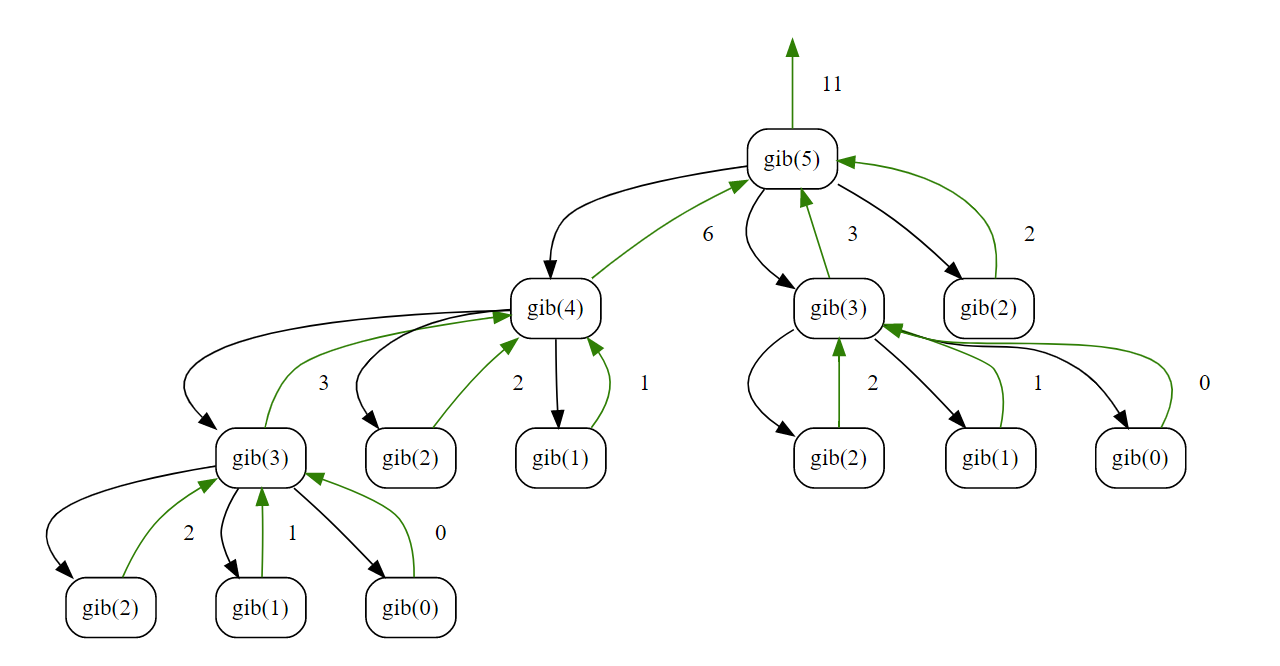
\includegraphics[width=0.7\textwidth]{gibonacci.png}

You could also build things from the ground up using intuition from the recursive leap of faith. 
\begin{itemize}
    \item \lstinline{gib(0)} takes one call because it's a base case. 
    \item \lstinline{gib(1)} takes one call because it's a base case. 
    \item \lstinline{gib(2)} takes one call because it's a base case. 
    \item \lstinline{gib(3)} takes four calls: one for the original call, one for \lstinline{gib(0)}, one for \lstinline{gib(1)}, and one for \lstinline{gib(2)}. 
    \item \lstinline{gib(4)} takes seven calls: one for the original call, four for \lstinline{gib(3)}, one for \lstinline{gib(2)}, and one for \lstinline{gib(1)}. 
    \item \lstinline{gib(5)} takes 13 calls: one for the original call, seven for \lstinline{gib(4)}, four for \lstinline{gib(3)}, and one for \lstinline{gib(2)}. 
\end{itemize}
This second method is much faster, especially for higher values of \lstinline{n}. 
\end{solution}
\end{blocksection}

\begin{questionmeta}
In general, I believe that drawing out call graphs can be confusing for students, especially for more difficult recursive problems. The whole idea behind recursion, after all, is that you don't have to worry about the dense tree of calls that result from a single call to a recursive function---you can just trust that the recursive calls you do make return the correct result and don't have to worry about how they specifically got that result. However, I believe that it is useful to do this sort of thing once because it demonstrates how recursion actually works in practice and why the recursion is valid and useful.

When teaching this problem, I recommend first going over the call tree. I would emphasize a few ideas. First, our base cases are at the bottom of the call graph, and every call eventually terminates at one of the base cases. They literally serve as the foundation of the tree. They are the ``truth'' upon which the function's validity for higher inputs rests. I would also point out that every call that's not a base case has three calls underneath it because each of these calls makes three recursive calls. Hopefully this makes the idea of recursion more concrete for the students and qualms perennial concerns that the logic behind recursion is circular. 

I would then going over the ``smarter'' way of doing the problem. I would point out how doing the problem in this way allows us to avoid the repetitive, confusing, and error prone work of considering every call in the function. I would note that if we tried to do the same thing with \lstinline{gib(1000)}, the graph would be untenable. The lesson I want them to walk away with is: abstracting away the huge number of calls is a valuable tool when working with recursion, and that they should try to avoid thinking about these calls if at all possible, as it only gets more confusing for more complicated functions. 
\end{questionmeta}